\section{Tarea 5 - Estudio experimental}
En esta parte se pide realizar un estudio experimental de medidas de tiempo para determinar qué
versiones de las anteriores son las más eficientes para unos datos concretos
\subsection{Condideraciones}
Utilizamos dos diccionarios (castellano e inglés) ambos contruidos mediante el texto de la declaración de derechos humanos.

Sobre estos creamos múltiples diccionarios con las N([20,100,500,2500]) palabras más frecuentes. Para ello sobrecargamos el constructor de la clase Suggest de maneara que acepte un path al corpus y un set de palabras ya creado.

Sobre cada uno de estos se crean N consultas([10,50,250,500,2500]). Estas son palabras pertenecientes al diccionario sobre las que se realizan unas perturbaciones aleatorias.

\begin{lstlisting}[caption=Función para crear perturbaciones aleatorias]
def perturbar(word):

    word = list(word)

    n_ops = random.randint(0, min(len(word)-1,MAX_PERTURBACIONES))

    for _ in range(0,n_ops):

        op = random.randint(0, 3)

        if op == 0: # borrar
            idx = random.randint(0,len(word)-1)
            word = word[:idx] + word[(idx+1):]
        elif op == 1: # cambiar
            idx = random.randint(0,len(word)-1)
            char = chr(random.randint(ord('a'),ord('z')+1))
            word[idx] = char
        elif op == 2: # trasposicion
            idx = random.randint(0,len(word)-2)
            tmp = word[idx]
            word[idx] = word[idx+1]
            word[idx+1] = tmp

    return "".join(word)
\end{lstlisting}

Estas consultas se realizan con todos los algoritmos desarrollados en las tareas previas.

Utilizamos el mismo diccionario y consultas con todos los algoritmos (datos apareados).

Repetimos 3 veces la medición de tiempo de cada algoritmo para cada talla de diccionario y consultas para luego poder explorar los resultados y ver que son consistentes y válidos.
\begin{lstlisting}[caption=medición de tiempos]
    start = time.time()
                        
    for consulta in tqdm(consultas,total=len(consultas),leave=False,desc='Consultas: ',position=4):
        _ = iss.suggest(consulta,distance=alg,threshold=STATIC_THRESHOLD)

    end = time.time()
    elapsed = end - start
\end{lstlisting}

\subsection{Resultados}

Una vez ejecutado el programa y realizado la medición de tiempos observamos que los tiempos medidos en las diferentes repeticiones con los mismos datos son parecidos, para ello obtenemos la media y desviaciones estándar.

Por ejemplo: para inglés, con talla de diccionario 20, talla de consultas 10 y el algoritmo Iterative intermediate obtenemos una media de 0.028734 y desviación estándard de 0.000572. Por lo que concluimos que los datos son válidos y procedemos a realizar la media de las diferentes repeticiones.

Realizamos el mismo procedimiento para los dos idiomas, inglés y castellano, observamos que el tiempo medidio con los mismos parametros son parecidos. Por lo tanto concluimos que los diferentes algoritmos se comportan igual en ambos idiomas y procedemos a realizar la media de ambas mediciones.

Finalmente, obtenemos para cada algoritmo una medición para cada talla de diccionario y talla de consulta.

Los resultados obtenidos muestran que todos los algoritmos escalan de manera lineal con la talla de consulta y de diccionario, y que el algoritmo más rápidos es Trie Levenhtein, seguido de Trie restricted.

\begin{figure}[h]
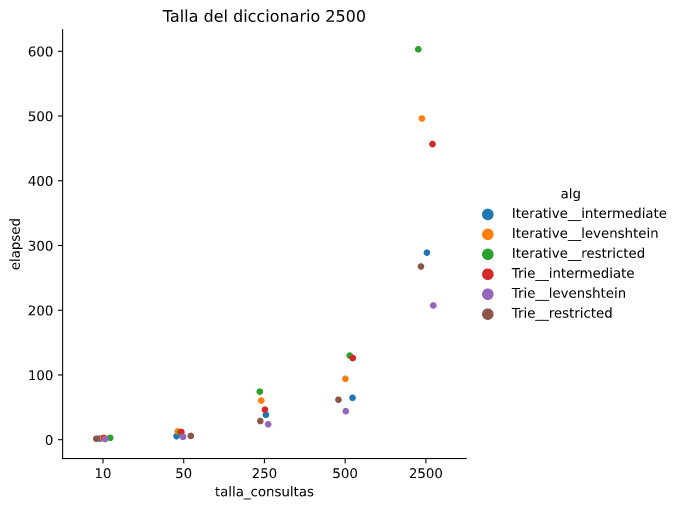
\includegraphics[width=15cm, height=10cm]{images/grafico.png}
\centering
\end{figure}

\newpage 